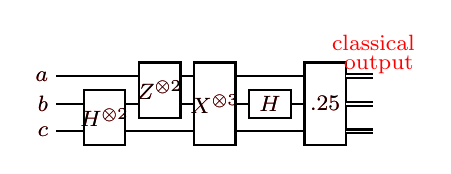
\begin{tikzpicture}[scale=.35]
    \footnotesize
    \visible<1>{
        \draw[red] (-1, 2.5) node[left] {$\ket{a}$};
        \draw[red] (-1, 1.5) node[left] {$\ket{b}$};
        \draw[red] (-1, .5) node[left] {$\ket{c}$};}

    \visible<2->{
        \draw (-1, 2.5) node[left] {$\ket{a}$};
        \draw (-1, 1.5) node[left] {$\ket{b}$};
        \draw (-1, .5) node[left] {$\ket{c}$};}


    \visible<2>{
        \draw[red, thick] (0,0) -- (1.5, 0) -- (1.5, 2) -- (0, 2) -- cycle;
        \draw[thick, red] (2+0,0+1) -- (2+1.5, 0+1) -- (2+1.5, 2+1) -- (2+0, 2+1) -- cycle;
        \draw[thick,red] (4+0,0) -- (4+1.5, 0) -- (4+1.5, 3) -- (4+0, 3) -- cycle;
        \draw[thick,red] (6,0+1) -- (6, 2) -- (7.5, 2) -- (7.5, 1) -- cycle;
        \draw[thick,red] (8+0,0) -- (8+1.5, 0) -- (8+1.5, 3) -- (8+0, 3) -- cycle;
        \draw[red] (.75, 1) node {$H^{\otimes2}$};
        \draw[red] (2.75, 2) node {$Z^{\otimes2}$};
        \draw[red] (4.75, 1.5) node {$X^{\otimes3}$};
        \draw[red] (6.75, 1.5) node {$H$};
        \draw[red] (8.75, 1.5) node {$\metersymbol{.25}$};}

    \visible<3->{
        \draw[thick] (0,0) -- (1.5, 0) -- (1.5, 2) -- (0, 2) -- cycle;
        \draw[thick] (2+0,0+1) -- (2+1.5, 0+1) -- (2+1.5, 2+1) -- (2+0, 2+1) -- cycle;
        \draw[thick] (4+0,0) -- (4+1.5, 0) -- (4+1.5, 3) -- (4+0, 3) -- cycle;
        \draw[thick] (6,0+1) -- (6, 2) -- (7.5, 2) -- (7.5, 1) -- cycle;
        \draw[thick] (8+0,0) -- (8+1.5, 0) -- (8+1.5, 3) -- (8+0, 3) -- cycle;
        \draw (.75, 1) node {$H^{\otimes2}$};
        \draw (2.75, 2) node {$Z^{\otimes2}$};
        \draw (4.75, 1.5) node {$X^{\otimes3}$};
        \draw (6.75, 1.5) node {$H$};
        \draw (8.75, 1.5) node {$\metersymbol{.25}$};}

    \visible<3>{

        \draw[red,thick] (-1, .5) -- (0, .5);
        \draw[red,thick] (1.5, .5) -- (4, .5);
        \draw[red,thick] (5.5, .5) -- (8, .5);
        \draw[red,thick, double] (9.5, .5) -- (10.5, 0.5);


        \draw[red,thick] (-1, 1.5) -- (0, 1.5);
        \draw[red,thick] (1.5, 1.5) -- (2, 1.5);
        \draw[red,thick] (3.5, 1.5) -- (4, 1.5);
        \draw[red,thick] (5.5, 1.5) -- (6, 1.5);
        \draw[red,thick] (7.5, 1.5) -- (8, 1.5);
        \draw[red,thick, double] (9.5, 1.5) -- (10.5, 1.5);


        \draw[red,thick] (-1, 2.5) -- (2, 2.5);
        \draw[red,thick] (3.5, 2.5) -- (4, 2.5);
        \draw[red,thick] (5.5, 2.5) -- (8, 2.5);
        \draw[red,thick, double] (9.5, 2.5) -- (10.5, 2.5);}

    \visible<4->{

        \draw[thick] (-1, .5) -- (0, .5);
        \draw[thick] (1.5, .5) -- (4, .5);
        \draw[thick] (5.5, .5) -- (8, .5);
        \draw[thick, double] (9.5, .5) -- (10.5, 0.5);


        \draw[thick] (-1, 1.5) -- (0, 1.5);
        \draw[thick] (1.5, 1.5) -- (2, 1.5);
        \draw[thick] (3.5, 1.5) -- (4, 1.5);
        \draw[thick] (5.5, 1.5) -- (6, 1.5);
        \draw[thick] (7.5, 1.5) -- (8, 1.5);
        \draw[thick, double] (9.5, 1.5) -- (10.5, 1.5);


        \draw[thick] (-1, 2.5) -- (2, 2.5);
        \draw[thick] (3.5, 2.5) -- (4, 2.5);
        \draw[thick] (5.5, 2.5) -- (8, 2.5);
        \draw[thick, double] (9.5, 2.5) -- (10.5, 2.5);}

    \visible<4>{
        \draw[red] (10.5, 3.7) node {classical};
        \draw[red] (10.7, 2.9) node {output};}

\end{tikzpicture}